\section{Evaluation}
\label{sec:experiment}


%In this paper, our task is to tackle commonsense reasoning problem in stories. 
%Given SCT as evaluation set, we can use any source data to learn human commonsense knowledge and reasoning ability. 
%We suppose the validation data has information leak for test set. The most classification methods which training or fine tuning with SCT validation set may learn the bias leak features, rather than commonsense reasoning ability
We first introduce some competing methods to be evaluated as well as
the datasets that they used for training and testing.
Then we present a preliminary analysis on the ROCStories dataset to invalidate
previous approaches that train or fine tune their models on the validation
set and we reconstruct a new dataset for training. Finally we conduct a comprehensive
evaluation of the competing methods to verify the effectiveness of our simplification method and 
the structured knowledge we incorporate.

%In this paper, our task is to tackle commonsense reasoning problem in stories. 
%Given SCT as evaluation set, we can use any source data to learn human commonsense knowledge and reasoning ability. 
%We suppose the validation data has information leak for test set. The most classification methods which training or fine tuning with SCT validation set may learn the bias leak features, rather than commonsense reasoning ability(\secref{sec:dataset}). We suggest to use a larger corpus with negative ending generated automatically. We also show our model parameter details in \secref{sec:details}, the comparison result with analysis in \secref{sec:result} and ablation study is in \secref{sec:ablation} .
\subsection{Baselines and Our Methods}
\label{sec:baselines}
The baselines which will be evaluated are separated into 2 parts.
First, as mentioned in ~\secref{sec:intro}, pretrained story representation 
helps with choosing the proper ending of a story. 
We apply our concept techniques on three typical 
models: DSSM, SKBC and BERT. 
These models are pretrained with different kinds of mechanisms
 and classification methods. We only take account of the 
 pretrained procedure. The other baselines which used the pretrained 
 methods are similar with these three models.

\textbf{[DSSM]}~\cite{mostafazadeh2016corpus} , semantic similarity 
between a pair of strings by representing them in a continuous semantic space.
In story ending prediction task, this model maps the four-sentence context and 
the fifth sentence into semantic vectors respectively considering the raw count of letter-trigrams without the order .
The context and an alternative are encoded through three hidden layers whose dimension are all 300. 
During test, DSSM chooses the alternative 
ending with the largest cosine similarity between its semantic vector and context's semantic vector.

\textbf{[SKBC]}~\cite{roemmele2017rnn}, uses Skip-thought~\cite{kiros2015skip} which 
can produce highly generic sentence representations and apply to many semantic classification problems.
Skip-thought is treated as the framework of encoder-decoder models. 
The architecture is GRU-GRU~\cite{hochreiter1997long} which 
has been shown to perform well on sequence modeling tasks.  
%We apply the simplification method and concept encoding.
We employ the same experimental 
setting as detailed in SKBC 
except for the addition of a dropout layer with 0.4 drop-rate before 1000-node GRU hidden layer. 
%We feed each simplified sentence of  a 5-sentence story into the dropout layer with 0.4 drop-rate. 
%Then we feed the dropout hidden state of each sentence 
%as a timestep into a single 1000-node GRU hidden layer.
A binary cross-entropy objective function is applied 
to maximize the probability of choosing the positive ending. 
All experiments use a batch size of 
200 and over 20 training epochs to optimize the model. 
To train concept sequence representation,  
we use a 2400-dimensional language model~\cite{kiros2015skip}\footnote{\url{https://github.com/ryankiros/skip-thoughts}} 
%from 98,161 unannotated ROCStories
from BookCorpus dataset~\cite{zhu2015aligning} which contains text from
11,038 books, primarily novels.


\textbf{[BERT]}~\cite{devlin2018bert}, without encoder-decoder archicheture, BERT exploits
transformer block~\cite{vaswani2017attention} which is a popular basic computational unit. 
There are several available pretrained BERT models which differ in how many
layers and parameters are used in the model (the basic version has 12-layer transformer blocks, 768 hidden-size, and 12
self-attention heads, totally 110M parameters; the large version has 24-layer transformer blocks, 1024 hidden-size, and
16 self-attention heads, totally 340M parameters). We apply our method on basic version which is trained with BookCorpus.

Our methods are applied on these models. 
For simplification method, we empirically fix the extra interval $\lambda$ to 1, 
because larger interval, while potentially helps discover more
concepts, may introduce noise. 
For example, in 
``Sally went home and wondered about her parents' marriage'', 
when $\lambda$ equals to 2 and 3, we will get ``go wonder'' and 
``go about'' incorrectly.

In addition, the structured knowledge representation takes the form of a 
300-dimensional vector from Numberbatch. 

For the second part of baselines, we compare
our method with other previous work on SCT task. 
These baselines are feature based, generative model or similar to the architecture of above three models including the 
state-of-art methods: 
%\KZ{I don't think we should introduce so many base lines here. Only present
%the baselines that you will improve on. I think u can have two sections,
%one is the set of baseline methods that uses the language model, which can be
%improved from our two techniques. The second is a set of other baselines that can
%be compared with us end-to-end, but these may not use language models.}

%\begin{description}

\textbf{[FES-JOINT]}~\cite{peng2017joint} combines the features of frame, 
entity and sentiment. This unsupervised joint model chooses the proper ending by 
calculating conditional probability.

\textbf{[SeqMANN]}~\cite{li2018multi} takes multiple shallow features into account, 
including POS tag, word embedding, character feature, 
sentiment negation and SemLM~\cite{peng2016two} features.

\textbf{[GMSA]}~\cite{guan2018story} generates the story ending through 
multi-source attention and brings in ConceptNet neighboring information.
We compare the similarity between the generated ending and alternatives.

\textbf{[CGAN]}~\cite{wang2017conditional} uses an generative adversarial 
network (GAN) which applies GRU to generate negative endings for 
training data augment.

\textbf{[SIMP]}~\cite{srinivasan2018simple} uses Skip-thought embeddings and 
encodes the entire story using a multi-Dense-layer classifier to determine the right ending.

\textbf{[GPT]}~\cite{radford2018improving} makes a big improvement by using 
multi-layer transformer to train a language model for text representation 
with linear fine tuning. GPT also use Transformer block as unit like BERT.

\textbf{[ISCK]}~\cite{chen2018incorporating} incorporates  sentiment and 
commonsense feature between the context and ending to 
\citeauthor{radford2018improving}'s text representation which can get a little improvement.


\textbf{[TransBERT]}~\cite{li2019story}, utilizes not only 
general language knowledge
 from large-scale unlabeled data but also  three
semantically related transfer tasks, including natural language
inference, sentiment classification, and next action
prediction, to pretrain and initialize BERT. 
% \end{description}

%In \textbf{our model}, the sentence representation contains text sentence 
%representation and commonsense structured representation. 
%n fact, our model is based on SKBC which consists of sentence encoding and 
%GRU network for classification. 
%Some experiments~\cite{roemmele2017rnn} have explores different embedding-based representations of the stories and different methods for generating negative examples.
%For {\bf our method}, %because Roemmele~\cite{roemmele2017rnn} has shown that training 
%sentence representation using ROCStories is almost as effective as
%using BookCorpus. 
%We used the same code and default parameters available
%at the above GitHub page. 

%As mentioned in \secref{sec:sentence simplification}, 
%For the tuning hyper parameter on story ending classifier. 
%We combine the sentence representations of the context and 
%final sentence into one sequence. 
%Each sentence representation is fed through a dropout layer 
%(drop-rate of 0.4) and then fed into a single 1000-node 
%GRU hidden layer. 
%The final hidden state value of two samples with same 
%context are given to a top feed-forward layer composed of one node  
%with softmax activation. 
%A binary cross-entropy objective function is 
%applied to train the network. 
\subsection{Dataset}
\label{sec:dataset}

%All datasets used in the experiments are documented in 
%\tabref{tab:datasets}.
%BookCorpus and ROCStories have been used to pre-train
%language models for this task in the previous work.

%\begin{table}[htbp]
%\small
%\setlength{\tabcolsep}{0.8mm}{
%\begin{tabular}{lllll} \hline
%\bf{Methods} & LM Train & Pred. Train & Validation & Test \\ \hline \hline
%DSSM & ROCS & -  & - &  SCT(T)\\ \hline
%FES-JOINT& NYT+ROCS & -  & - &  SCT(T)\\ \hline
%SeqMANN & ROCS & ROCS*(Tr)& ROCS*(V)& SCT(T)\\ \hline
%SIMP & BC & BC(Tr)& ROCS*(V)& SCT(T) \\ \hline
%SKBC & BC & BC(Tr)& ROCS*(V)& SCT(T)\\ \hline
%CGAN & ROCS & - & - &  SCT(T)\\ \hline
%GMSA & ROCS & - & - & SCT(T)\\ \hline
%GPT & BC &  ROCS*(Tr)& ROCS*(V)& SCT(T)\\ \hline
%ISCK & BC & ROCS*(Tr) & ROCS*(V) & SCT(T) \\ \hline
%BERT & BC+WIKIPEDIA &  ROCS*(Tr)& ROCS*(V)& SCT(T)\\ \hline
%TransBERT & BC+WIKIPEDIA &  ROCS*(Tr)& ROCS*(V)& SCT(T)\\ \hline
%Ours(BC) & BC &ROCS*(Tr) &ROCS*(V) & SCT(T) \\ \hline
%Ours(ROCS) & ROCS &ROCS*(Tr) &ROCS*(V) & SCT(T) \\ \hline
%\end{tabular}}
%\caption{Datasets used by different methods for training
%language model and the ending prediction, for validation and
%for test
%(BC = BookCorpus, NYT = New York Times \protect\footnotemark ,
%ROCS = ROCStories, ROCS* = ROCStories annotated with positive  by AMT and 
%negative endings by our generation approach,
%SCT=Story Cloze Test, T = test dataset, V = validation dataset, Tr = training dataset)}
%\label{tab:datasets}
%\end{table}
%\footnotetext{Available at \url{https://catalog.ldc.upenn.edu/LDC2008T19}}

To train the story ending prediction models, many previous works
used the SCT validation split which contains 1871 annotated items,
and achieved very good results.
We argue that the validation set cannot be used as training resource because
it suffers from human-authorship bias~\cite{sharma2018tackling}. 
Analogously, research~\cite{niven2019probing}
has shown that the result of BERT on Argument Reasoning
Comprehension Task~\cite{habernal2017argument} entirely
relies on exploitation of spurious statistical cues in the dataset. 
The following preliminary experiment shows the existence of bias cues in SCT. 

ROCStories and their negative endings in SCT are solicited
on Amazon Mechanical Turk (AMT). We found that the endings
contain significant information leak. For example, \tabref{tab:hate}
shows a feature (the word ``hate'') that is overwhelmingly found 
in the negative endings.
This means that by extracting such features from two endings, an algorithm
may be able to predict the correct ending with high accuracy. 


%SCT=Story Cloze Test, T = test dataset, V = validation dataset, Tr = training dataset

\begin{table}[th!]
\small
\centering
\begin{tabular}{lccc}
\hline
\textbf{Dataset}& Pos ending& Neg ending &Total\\
\hline
Validation set & 3  & 70 &73\\
Test set          & 4  & 69 &73\\
\hline
\end{tabular}
\caption{Frequency of word ``hate'' appearing in the positive and 
negative endings of SCT Validation set(SCT(V)) and Test set(SCT(T))}
\label{tab:hate}
\end{table}

\begin{table}[th!]
\small
\centering
\begin{tabular}{lcc}
\hline
\textbf{Model}& SCT(V) (\%) &ROCS*(Tr) (\%)\\
\hline
%~\citeauthor{end:predict}(~\citeyear{end:predict})&72.5\\
SIMP& 72.60 &59.86\\
SKBC&72.76&58.18\\
GPT& 77.77 &57.93\\
$\text{TransBERT}_\text{BASE}$&79.0&54.52\\
$\text{TransBERT}_\text{LARGE}$&75.84&54.30\\
\hline
Human& 62.40&62.40\\
\hline
\end{tabular}
\caption{Test accuracies of various models trained on the endings only
from SCT(V) and ROCS*(Tr)}
\label{tab:end}
\end{table}


We re-evaluated several top-performing algorithms and our method
by adapting them to train {\em only on the endings} in the validation set(SCT(V)). 
The result on the test set of SCT is shown in \tabref{tab:end}. 
As a baseline, we include the human performance, which is the average
accuracy of 5 human annotators who are not
trained on the validation set but use their commonsense only. The fact
that human score is substantially worse than some of the ``top'' algorithms
indicates that these algorithms are not using ``commonsense'' but rather
the patterns leaked in the training data. $SCT_v1.5$~\cite{sharma2018tackling}
is a recently released revised version in order to reduce the 
human-authorship biases in SCT. However the ending-only results for
$SCT_v1.5$ is still higher than human~\cite{sharma2018tackling}. 
Therefore this dataset does not necessarily solve the problem. 
Nevertheless, we show the result of our model on $SCT_v1.5$(~\secref{sec:result}).

Therefore, in this paper, we choose to create a new training dataset
by automatically augmenting ROCStories corpus with negative endings.
It is unnatural for human to come up with negative
endings for a story, while most people have no problem predicting a positive
one.
%Therefore we propose to generate negative endings automatically . 
We follow ~\cite{roemmele2017rnn} and generate negative examples for the 98161 stories in ROC training set 
by Random and Backward 
%\eve{further explanation of Backward method or give citation?} 
 method with 4:2 proportion. Then we randomly choose one 
from the six alternative endings to ensure the balance of positive and negative data. 
The resulting dataset is called ROCS*.
Finally, we split ROCS* 4:1 into training (ROCS*(Tr)) and 
validation set (ROCS*(V)). 
In  \tabref{tab:end}, we can find the machine learning with only endings performs
worse than human on our reconstructed training dataset which is more valid for training. 
This dataset for training remedies the bias information leak to some extent.
Note that all the training dataset, 
validation dataset, test dataset in the following are referred as our new dataset: ROCS*(Tr),
ROCS*(V) and SCT(T).

%ROCStories corpus consist of 98,161 five-sentence 
%stories without negative ending . 


\begin{table}[th!]
\small
\centering
\begin{tabular}{lccc}
\hline
\textbf{Dataset}&Total story&Context zeros& Ending zeros  \\
\hline
%~\citeauthor{end:predict}(~\citeyear{end:predict})&72.5\\
Training& 157058 &0&26\\
Validation&39264&0&8\\
Test&3742&0&0\\
\hline
\end{tabular}
\caption{The total number of stories (context and a positive or negative ending) and  the number 
of the stories whose context or ending contains zero concept 
in Training dataset, Validation dataset and Test dataset }
\label{tab:size2}
\end{table}

We choose ConceptNet as our simplification corpus mainly for the high coverage of
commonsense knowledge which is constructed from multi-source, such as 
WordNet, DBPedia, and OpenCyc. 
%Our approach is dependent on simplifying the sentence
%by extracting key concepts and mapping them to ConceptNet. 
Given the new dataset, if none of the concepts in a sentence 
is found in ConceptNet, this problem is called 
Out of Vocabulary (OOV) on concepts. 
However, in \tabref{tab:size2}, our preliminary study shows
 that fewer than 0.020\% and 0.017\% of the ending sentences contain no concept at all in training 
 and validation dataset, which shows ConceptNet covers comprehensive domain of concepts.
%The second reason for why we don't use validation for training is the quantity of the SCT validation set. It only contains 1871 stories. Most of the previous research split 1497 stories for training and 376 stories for validating. Intuitively, learning the ability of commonsense reasoning in story from about 1500 stories is impossible. \KZ{Can we have a bit of result here to support thisclaim? There are two reasons u present here but the second one is too light-weight.} 

%\KZ{The following 3 paragraphs are too verbose. Cut to just one short para!} 
%The motivation of this task is to learn large quantity of commonsense knowledge and reasoning ability. Given SCT evaluation dataset, most of previous research are trained with negative examples. However, writing large amount of negative examples manually is too expensive. At the same time, human writing  always take in human bias, just as the example in ~\tabref{tab:end}.
%
% Because story ending should initially have two features: probability equivalence and coherence. In ROC validation set, some endings are illogical in commonsense, for example, the ending ``the glasses fixed his headaches immediately'' is much more likely than``the optometrist gave him comfortable sneakers''. Of course, the second ending is wrong, but the inequity  have nothing to do with story prediction task. We choose the endings from other story which are equal in probability. In addition, the backward approach improves the degree of semantic coherence with the context sentences. 
%
%We shuffle and split the 98161 story set with negative endings into 5 folds, one for  Valid-RB (new validation set) and the rest for Train-RB (new training set). The test set is the same with SCT. The accuracy for models train on Train-RB endings is shown in  ~\tabref{tab:end}. By comparison with \tabref{tab:end}, the scores imply the models can not get a good model with only endings. Train-RB strongly reduces the ending bias.
%
%
%%\KZ{You need to add a paragraph to talk about how you evaluated human
%performance. Who participated in these test, how were they evaluated.
%Maybe the same humans did the test for the endings only. So we need to
%think about where to put this paragraph. Here or earlier when you talk
%about ending only.}
 
\subsection{End-to-end Results}
\label{sec:result}

We first show the end-to-end results of the three baselines 
with simplification and concept encoding methods. Then we 
evaluate other models trained with new dataset on SCT.

\begin{table}[th]
 \small
\centering
\setlength{\tabcolsep}{0.7mm}{
\begin{tabular}{lcccc}
\hline
$\textbf{Model}$ &Orignal (\%)&Simp(\%)&CE(\%)&Simp+CE (\%)\\
\hline
\hline
DSSM& 54.04&58.79&54.0&58.2\\
SKBC&64.70&68.13&65.12&\bf{69.7}\\
$\text{BERT}_\text{BASE(ours)}$&56.54&57.34& 59.43&60.24\\
\hline
\end{tabular}}
\caption{End-to-end accuracy on SCT test set with simplification and concept encoding methods. 
Original=baseline, Simp=simplification method, CE=concept encoding method
}
\label{tab:main}
\end{table}

\tabref{tab:main} shows  all the three typical pretrained 
story representation models benefit from our simplification 
and concept encoding methods. 
SKBC and DSSM get 3.43\% and 4.75\% which are great improvement with simplification. 
$\text{BERT}_\text{BASE}$ get 0.8\% improvement with simplification and 
2.89\% with concept encoding method which are both compared with original model. 
It is because BERT contains Transformer unit which is attention mechanism. 
BERT can learn the informative weight from pre-training. Our simplification can even 
help with reducing the weight of less informative words for BERT. 

% Then we apply two encoding aspects: 
%simplification language model encoding 
%on three typical pretrained language models to 
%verify that each semantic aspect contributes to the ending prediction model.

\begin{table}[th]
 \small
\centering
\begin{tabular}{lc}
\hline
$\textbf{Model}$ & Acc (\%))\\
\hline
\hline
DSSM(implement)& 54.04\\
GMSA& 61.20\\
CGAN& 60.90 \\
SeqMANN(implement)& 59.74\\
SIMP(implement)&61.09\\
FES-LM(implement)&61.60\\
ISCK(implement)& 62.21 \\
GPT(implement)& 63.46\\
SKBC(implement)&64.70\\
$\text{BERT}_\text{BASE(ours)}$(implement)&56.54\\
$\text{BERT}_\text{BASE}$(implement)&61.46\\
$\text{BERT}_\text{LARGE}$(implement)&64.67\\
$\text{TransBERT}_\text{BASE}$(implement)&61.46\\
$\text{TransBERT}_\text{LARGE}$(implement)&61.89\\
\hline
SKBC+Simp+CE(ours)&\bf{69.7}\\
%\hline
%DSSM+simp(ours)&58.79&+4.75\\
%SKBC+simp(ours)&68.13&+3.43\\
%$\text{BERT}_\text{BASE*}$+simp(ours)& {57.34}&+0.8\\
%\hline
%DSSM+ce(ours)&54&-0.04\\
%SKBC+ce(ours)&65.12&+0.42\\
%$\text{BERT}_\text{BASE*}$+ce(ours)& 59.43&+2.89\\
%\hline
%DSSM+simp+ce(ours)&58.2&+4.16\\
%SKBC+simp+ce(ours)&\bf{69.7}&+5.0\\
%$\text{BERT}_\text{BASE*}$+simp+ce(ours)&60.24&+3.7\\
%
\hline
Human& 100\\
\hline
\end{tabular}
\caption{Experimental results of story ending prediction on SCT}
\label{tab:all-models}
\end{table}

%We use the same training data for
%all supervised or semi-supervised approaches in this section. 
%\footnote{Some of the algorthms compared here may have reported better
%accuracies than those reported here, but that's because they were trained
%on the validation set.}
\tabref{tab:all-models} shows the results of other previous research on our new training 
and validation dataset in ~\secref{sec:dataset}. Most of baseline models are implemented in strict accordance with the settings in the original papers.  
We can find the best previously reported result is from SKBC, whose accuracy is 64.7\%.
We implement the same BERT model and get a secondary score of 64.67\%
second-ranked with large version. 
Our $\text{BERT}_\text{BASE}$ does not preform as good as the basic version because we retrain the 
language model with BookCorpus only.  Though larger corpus, such as  Wikipedia, can get a better result,
we only expect to show the effectiveness of our simplification and concept encoding methods. 
SKBC with our methods achieves accuracies of 69.7\%, which is the best in our experiments. 
It performs better than any other models. Being the state of art is not our first concern. 
Maybe other models with our methods can get better 
results.
%The ending prediction results with BC and ROCS are nearly identical  
%which is consistent with Roemmele~(\citeyear{roemmele2017rnn})'s research.
%We also get the SOTA performance of 68\% on the newly 
%released $SCT_v1.5$ blind test dataset by training the language model on BC, 
%which is not shown in this table.  
%Unless otherwise noted, our model is trained on ROCStories.
Human performance is 100\% and can be used as an 
upperbound~\cite{mostafazadeh2016corpus}. 
%The models are divided into two
%categories, either using 
%the generated negative endings for binary classification or not at all. 
All results are averaged from
5 independent runs. 
%Note that the numbers reported 
%are not directly comparable with those in literature~\cite{srinivasan2018simple,roemmele2017rnn,li2018multi,radford2018improving,chen2018incorporating} as we reconstruct 
%training and validation set for binary classification methods which has been
%described in \secref{sec:dataset}.


%DSSM achieves an accuracy of 58.5\%, it simply uses a deep structured semantic model to learn representations for both context and endings and chose ending by calculating the similarity between the context and ending representation. GMSA model is a generative model, which takes in structured ConceptNet knowledge. Though it is not used for choosing endings, we compute the similarity between the generated ending and two alternatives and get 61.2\% for comparison. The semi-supervised models all rely on negative endings. CGAN achieves 60.9\% accuracy by generating negative endings with generator in GAN. The goal of their generator network is to generate a fake sentence and deceive the discriminator to take it as real target. SeqMANN achieves 59.74\% accuracy incorporating with many language features,. GPT make great achievement training on SCT validation set and get 63.46\% accuracy training on Train-RD. This model use transformer train a language model and fine tune to train a classifier. ISCK which is the best when using SCT validation set for training further improves the performance to 62.21\%. It combines the sentence representation of GPT, sentiment feature and commonsense similarity feature between the context and endings. SKBC the state-of-art in former models we reproduce achieves 64.7\% accuracy with skip-thought sentence representation and RNN classifier. We suppose GPT and ISCK learn the representation of sentence itself. Skip-thought model encode the sentence representation with former and later sentence information. This kind of information is more efficient in commonsense reasoning. SIMP is even more simple for only using dense layer to classify the story lines on 61.09\% accuracy. 
 
%Our model outperforms all the baselines. In fact we 
%logged 5\% improvement over
%Similar to SKBC model, we represent the story sentence with 
%low-dimension vectors and train a classifier with GRU model. 


%Also, for the record, our model correctly predicts the question in
%\figref{fig:story} while other strong competitors such as SIMP, GPT and ISCK
%failed.

%\KZ{Add one or two example stories in which we did correct but other algorithms
%failed. Give a brief analysis to show why our method do better 
%than this example. Actually here it would be ideal if our driving example
%can be used. That is, indeed our method predicts correctly while the major
%competitors failed.}
 
\subsection{Different Simplification Strategies}
\label{sec:simplify}
%Previous work on predicting ending of a story mainly divided into two directions. The first direction aims to generate ending for given context with generative language model~\cite

\begin{table}[th!]
\small
\centering
\begin{tabular}{lcc}
\hline
\textbf{Event Type} & Acc w/o CE (\%) & Acc w/ CE (\%)\\
\hline \hline
All Words(SKBC)& 64.70 & 65.12\\
\hline
5-TUPLE&55.12 &57.83\\
FES&60.12 &63.66\\
%No Events & - & 63.70 \\
Simp(ours)& 68.13 &{\bf 69.70} \\
\hline
\end{tabular}
\caption{The effect of using different types of events for simplification
on SCT}
%No Events = concept embedding only, 
%Simp = simplified sentence embedding}
\label{tab:sse}
\end{table}

\begin{table}[th!]
\small
\centering
\setlength{\tabcolsep}{0.7mm}{
\begin{tabular}{lccc}
\hline
%\textbf{Dataset}&Words&Concepts& Simplified words\\
%\hline
%Training   &10.03&3.79&5.17\\
%Validation&10.03&3.79&5.17\\
%Test         &9.57&3.59&4.90\\
\textbf{Event Type}& Before & Events & After \\
\hline
5-TUPLE&10.02&1&3.43\\
FES&10.02&1.52&8.95\\
Simp(ours)&10.02&3.78&4.90\\
\hline
\end{tabular}}
\caption{Effects of simplification using different types of
events on the length of the word sequence. 
Before = avg. num of words before simplify,
After = avg. num of words after simplify, Events = avg. num of events
extracted.}
\label{tab:size}
\end{table}


%\begin{table}[th!]
%\small
%\centering
%\begin{tabular}{lc}
%\hline
%\textbf{Types of information} & Acc (\%)\\
%\hline \hline
%SKBC (whole sentence embedding)& 64.70 \\
%\hline
%\hline
%\end{tabular}
%\caption{The effect of incorporating with concept embedding on SCT}
%\label{tab:ce}
%\end{table}

Understanding a story requires understanding sequences of events. 
%It is thus vital to model mantic sequences in text. 
To evaluate the ability of 
simplification methods on story ending prediction task, we make comparison with
 two types of event representation, 5-TUPLE~\cite{pichotta2016learning} and FES~\cite{peng2017joint}
  which rely on dependency parsing or SRL . 
  %We employee the same settings with \textbf{our model}, 
  %except for the sequence modeling methods.
  5-TUPLE represents an event as a 5-component tuple $(v, e_s, e_o, e_p, p)
  $\footnote{We  parse ROCStories with Stanford CoreNLP tools for 5-TUPLE.}, 
  where $v$ is a verb lemma which can not be $null$, $e_s$, $e_o$ and $e_p$ are nominal 
  arguments standing in subject, direct object and prepositional 
  relations respectively and $p$ is the preposition relating $v$ and $e_p$. 
The other event representation FES jointly models different aspects of 
semantic knowledge: frames\footnote{Semantic frames 
are derived from semantic role labeling annotations built upon PropBank frames. }, 
entities and sentiments. 
Different from the original paper, we represent all three aspects 
as \textit{string} instead \textit{vector} (e.g. \textit{POSITIVE} 
label vs one-hot vector for sentiment).

\tabref{tab:sse} shows the effectiveness of these simplification methods trained 
on the same model architecture of SKBC. 5-TUPLE only 
achieves 55.12\% which omits too much information. In \tabref{tab:size}, 
The average number of words is only 3.43. Though FES brings in more information, 
the extraction of  frames is a pipelined process and suffers from low accuracy.
%We conduct an ablation study on the proposed model to evaluate 
%the effectiveness of each feature. Results using only one type of 
%embedding for sentence representation are shown in \tabref{tab:ablation}. 
%The representation with simplified sentence achieves 3.43\% improvement 
%over the sentence embedding of the original sentence. It also shows that
%sentence simplification is a more effective feature than concept embedding. 
\subsection{Effects of Concept Embeddings}
\label{sec:ce}
\tabref{tab:sse} also shows all event sequence representations can benefit from 
the incorporation with  concept encoding which is pretrained on ConceptNet. 
The result for Simp and Simp+CE shows that the relation between concepts can introduce extra 
knowledge which can not 
be learnt from language model.

\subsection{Training Data Size}
\label{sec:datasize}

\begin{figure}[th!]
\centering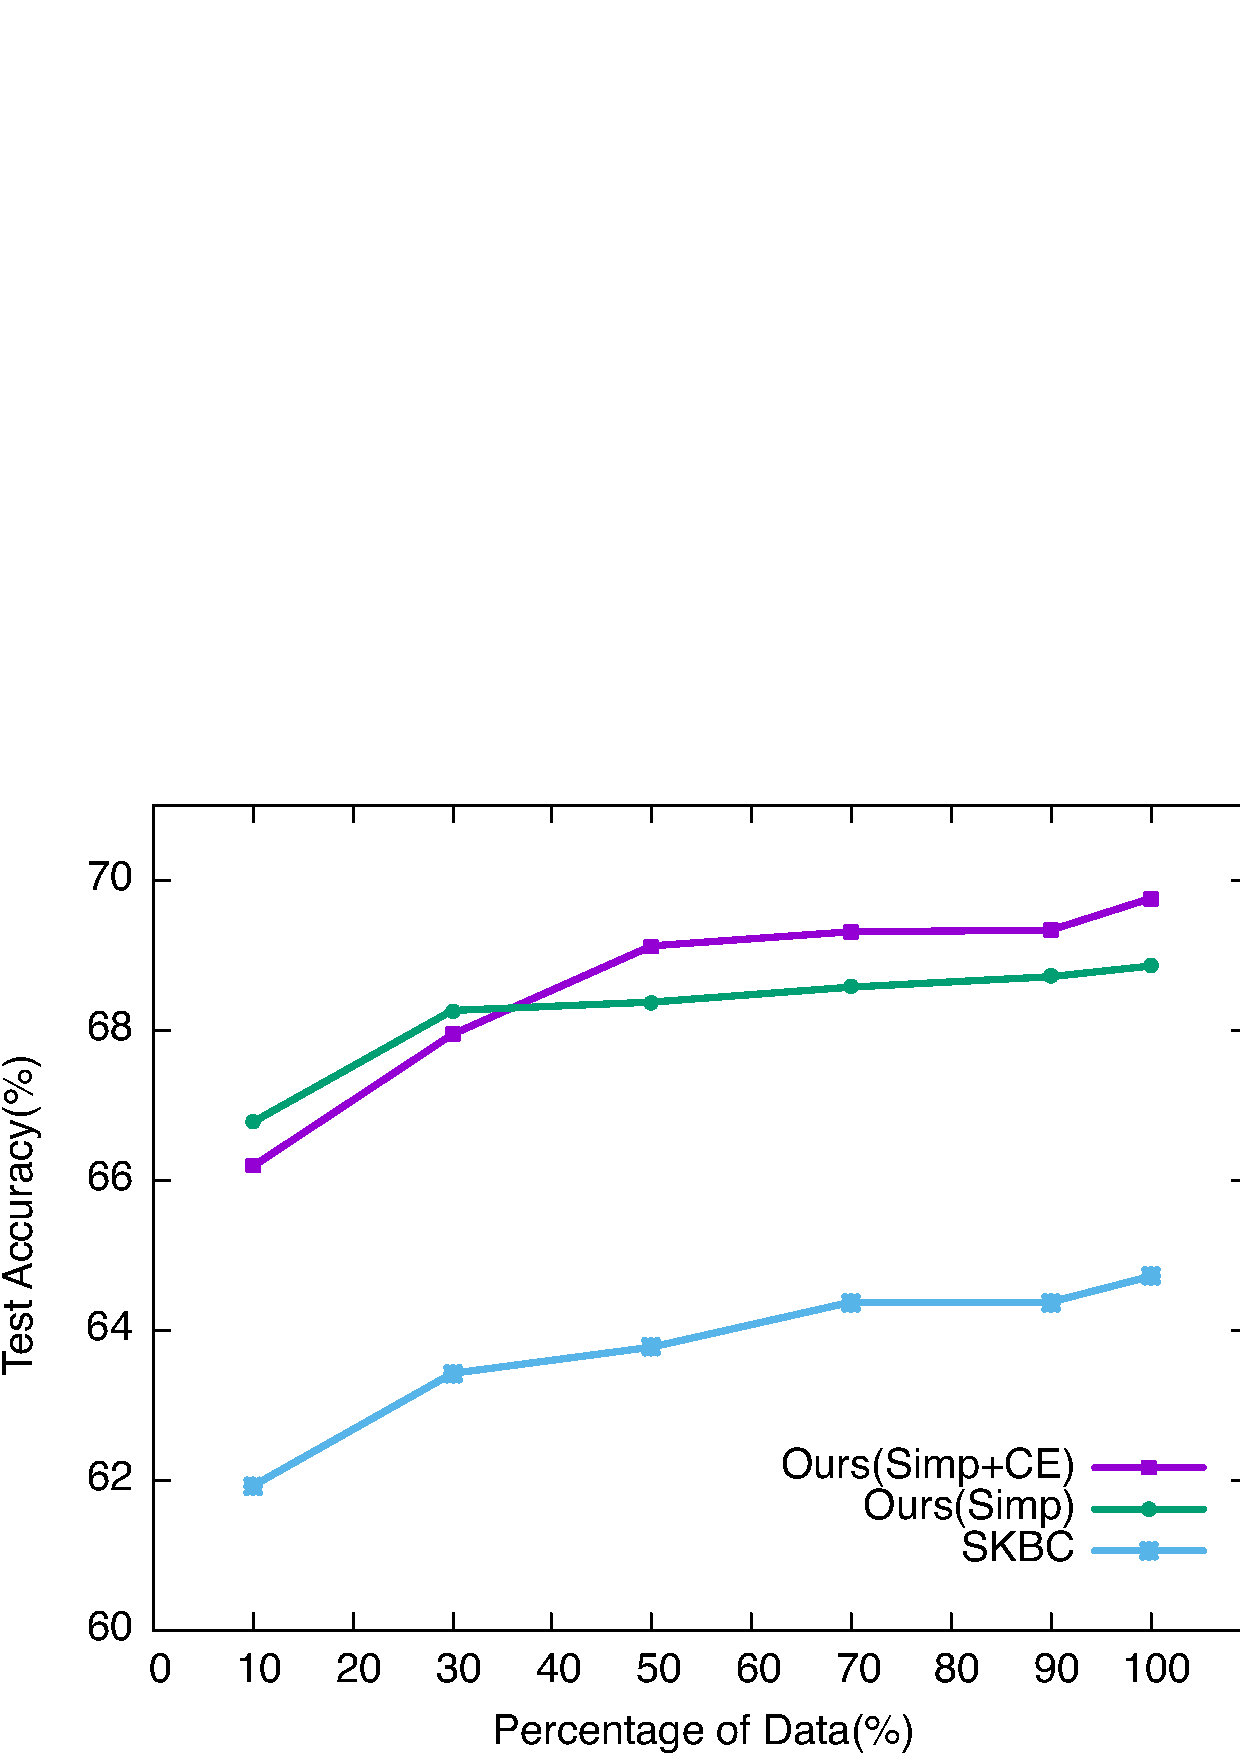
\includegraphics[width=0.7\columnwidth]{pictures/trend}
\caption{Accuracies over train data size}\label{fig:trend}
\end{figure}

In \figref{fig:trend}, we compare the models' capability given increasing
amount of training data (ROCS*(Tr)). The first observation is that our two models (Simp
and Simp+CE) both perform well even with very little training data. In fact,
given 10\% of the data, they already achieve higher accuracies than SKBC using
the whole data. The second observation is that compared with SKBC, our models
get improved more quickly as the training data grows, which is indicated by
the steeper slope from 10\% to 50\% of the data. 
Finally, when comparing the effects with or without the concept embedding, 
we can see that without structured knowledge,
the model is unable to take advantage of more training data. 

\subsection{Training Time}
\label{sec:time}
Except for the improvement on end-to-end accuracy, the simplification 
can also take a one-third reduction in time.
The improvement in efficiency comes from fewer tokens in sentences 
and smaller vocabulary.
% \eve{what is 'various of data'? 'various' should be 'variousness'}
There exist 43,095 unique words in all ROCStories and 
19,455 unique words in simplified key tokens extracted from ConceptNet. 
This greatly reduces the vocabulary size.
%In addition, the structured commonsense feature 
%also brings in extra commonsense knowledge. 
%the best result for WSE is 64.7\% with all data. 
%Though accuracy is still growing, the growth is slowing down. 
%With the limited training data, our model performs much better. 
%The reducing of noise and variance improves sentence representation quality. 
%The concepts embedding from , though can't give all the sentence information to the representation, helps improve the accuracy to 69.7\% which is the state of art in model comparison. The results suggest neither of these two kind of sentence embedding is sufficient to represent the commonsense knowledge and the combination can give the best performance.
